\chapter{Biblioteca Digital do Participa.br}
\label{cap:bibparticipabr}

Nesse capítulo será apresentado alguns resultados dos levantamentos iniciais sobre os mecanismos formais de participação, além de apresentar um primeiro protótipo sobre a biblioteca digital do Participa.br. Para esse primeiro protótipo, os metadados considerados serão apresentados na seção \ref{sub:metadadospbr}. Mais adiante uma proposta para interoperabilidade do Participa.br (Noosfero) e a biblioteca digital através de um plugin que implementa o protocolo OAI-PMH é visto na seção \ref{sec:interparticipa}. Já o primeiro protótipo da biblioteca digital de participação social é visto na seção \ref{sub:prototipo_biblioteca}.

Também constam recomendações e sugestões sobre preservação de artefatos digitais visando uma sobrevida maior, e beneficiando não somente documentos textuais, mas todo e qualquer tipo de informação multimídia (áudio, vídeo, imagem, etc.).

\section{Arquitetura da Informação sobre Participação Social}

Atualmente não existe um lugar centralizado para os usuários buscarem informações sobre os mecanismos formais de participação. Cada órgão possui seu próprio repositório de informações, disponibilizados em diversas formatos digitais, sendo elas: planilhas, documentos, páginas HTML, entre outros. Muito desses órgãos disponibilizam informações desatualizadas e incompletas, outros já disponibilizam os dados de formas estruturadas e completas como no caso do Conselho Nacional de Saúde. 

Aliado ao crescente número de mecanismos formais de participação durante a última década, ficou evidente que encontrar informações sobre esses mecanismos se torna dispendioso. Por isso é necessário criar um canal onde os usuários possam acessar todos os dados de maneira centralizada, e que as informações sobre os mecanismos formais possam estar sempre atualizadas, tudo isso dentro do Participa.br.

Para criação desse canal centralizado para disponibilização dos mecanismos formais de participação foi feito um primeiro levantamento. Esse levantamento levou em consideração as informações disponibilizadas nos diversos portais dos canais de participação (mais especificamente sobre conselhos, conferências e ouvidorias) e nas entrevistas que foram realizadas durante o período de confecção da primeira versão desta monografia.

Após esse levantamento inicial, foi notado que os sites são muito heterogêneos e que a estrutura assumida por cada canal é peculiar àquele site. De um modo geral, as informações de participação social incorporam páginas web e arquivos textos com a maior parte das informações. Além dessa forma, muitos sites contém arquivos multimídia contendo áudio, vídeo e imagens como documentários sobre as reuniões dos conselhos, palestras, entre outros, que podem ser colocados para visualização dos usuários.

É importante ressaltar que, num primeiro momento, para apresentação do protótipo, foram considerados apenas alguns objetos digitais construídos especialmente para essa biblioteca digital cujos conteúdos são exatamente as informações essenciais do canal de informação, tais como o URL, os dados do gestor e outras informações relevantes. Portanto, esse foi o nível de granularidade definido para o objeto digital nesse primeiro protótipo de biblioteca digital.


\section{Metadados de Participação Social}
\label{sub:metadadospbr}

A fim de atender ao propósito dessa pesquisa, foi feito um levantamento nos principais mecanismos formais de participação, a fim de identificar quais seriam os metadados relevantes a serem incluídos na biblioteca digital do Participa.br. Além desse levantamento em sites, alguns gestores foram consultados para que opinassem sobre que tipo de informações eles gostariam de ver respondidas com a biblioteca digital. O resultado desse levantamento permitiu elencar os metadados que estão apresentados nas Tabelas \ref{tab:metadata_dc_conselho} a \ref{tab:metadata_pbr_ouvidorias} para conselhos, conferências e ouvidorias, considerados os principais canais de participação para efeito de teste da biblioteca digital que está sendo proposta.

Na tabela \ref{tab:metadata_dc_mecanismo} serão apresentados os metadados significativos para conselhos, conferências e ouvidorias que tem uma correlação com metadados do padrão Dublin Core.

\newcolumntype{'}{!{\vrule width 2pt}}
\makeatother 

\begin{table}[H]
	\begin{center}
	\caption{Metadados Participa com Relação DC para Conselhos, Conferências e Ouvidorias}
    \begin{tabular}{'l|p{9cm}'}\thickhline
    \rowcolor[HTML]{BFBFBF}
    \multicolumn{1}{!{\vrule width 2pt}c!{\vrule width 1pt}}{\textbf{METADADO}} & 
  \multicolumn{1}{!{\vrule width 0pt}c!{\vrule width 2pt}}{\textbf{DESCRIÇÃO}} \\ \noalign{\hrule height 3pt}
    dc.title & Nome do mecanismo formal de participação \\ \hline
    dc.creator & Órgão o qual aquele canal formal faz parte. \\ \hline
    dc.subject & Palavras chaves que relacionam ao canal formal. \\ \hline
    dc.description & Uma pequena descrição, finalidade ou objeto o qual aquele mecanismo formal está ligado.\\ \hline
    dc.date & Data de criação do canal de participação. \\ \hline
    dc.type & Tipo de caráter que o canal de participação possui (representativa, consultiva, deliberativa, participativa, etc.). \\ \hline
    dc.identifier & URL/URI do canal de participação. Sítio Eletrônico onde se encontra a página do canal formal de participação. \\ \hline
    dc.language & Linguagem utilizada descrição do canal formal de participação (previsão para outras linguagens no futura.) \\ \hline
    dc.relation & Define ligação entre canais formais. \\ \hline
    dc.rights & Tipo de licença para divulgação do conteúdo daquele canal. \\ \noalign{\hrule height 2pt}
    \end{tabular}
    \end{center}
    \label{tab:metadata_dc_mecanismo}
\end{table}

Como o padrão Dublin Core não foi suficiente para mapear todas as referências necessárias para os artefatos digitais, foi definida uma tabela específica para cada um dos três tipos de mecanismos formais de participação, usando um conjunto de metadados específico, identificados com o prefixo pbr como uma alusão ao projeto Participa.br. Esses metadados específicos possuem a desvantagem de não serem interoperáveis fora do contexto dos canais de participação social que estiverem conectados à rede de bibliotecas digitais planejada para o Participa (essa discussão será feita mais adiante na seção \ref{cap:extbibparticipa}), no entanto, eles descrevem melhor as demais referências que não foram mapeadas no Dublin Core.

Na tabela \ref{tab:metadata_pbr_conselho} estão os metadados do Participa.br, que não possuem relação com o Dublin Core para conselhos.

\begin{table}[H]
\begin{center}
    \caption{Metadados Participa para conselhos}
    \begin{tabular}{'l|p{9cm}'}\thickhline
    \rowcolor[HTML]{BFBFBF}
    \multicolumn{1}{!{\vrule width 2pt}c!{\vrule width 1pt}}{\textbf{METADADO}} & 
  \multicolumn{1}{!{\vrule width 0pt}c!{\vrule width 2pt}}{\textbf{DESCRIÇÃO}} \\ \noalign{\hrule height 3pt}
    pbr.sigla & Sigla do mecanismo formal de participação \\ \hline
    pbr.competencia & Competências e atribuições a qual o conselho responde, geralmente regidas em lei. \\ \hline
    pbr.composicao & Composição entre os membros de um conselho, também geralmente são regidas em lei (Por exemplo: membros da sociedade civil, membros da esfera pública). \\ \hline
    pbr.escolha & Forma de escolha dos membros (Por exemplo: votação, indicação, etc.). \\ \hline
    pbr.mandato & Nome das pessoas que estão fazendo parte do conselho em um determinado tempo. \\ \hline
    pbr.legislacao & Todas as leis (Leis, decretos, portarias, etc.) que estão relacionados aquele conselho. \\ \hline
    pbr.endereco & Esse metadado possui informações sobre o endereço físico a qual aquele conselho está instalado (Bairro, Cidade, CEP, Rua, etc.) e também inclui informações sobre telefone e e-mail do conselho. \\ \hline
    pbr.dtreuniao & Data de reuniões, audiências, etc. \\ \noalign{\hrule height 2pt}
    \end{tabular}
    \label{tab:metadata_pbr_conselho}
\end{center}
\end{table}

%Tabela 3.2 - Metadados Participa para conselhos

Na tabela \ref{tab:metadata_pbr_conferencias} estão apresentados os metadados Participa.br para conferências e que não tem uma correlação com metadados do padrão Dublin Core.

\begin{table}[H]
\begin{center}
    \caption{Metadados Participa para conferências}
    \begin{tabular}{'l|p{9cm}'}\thickhline
    \rowcolor[HTML]{BFBFBF}
    \multicolumn{1}{!{\vrule width 2pt}c!{\vrule width 1pt}}{\textbf{METADADO}} & 
  \multicolumn{1}{!{\vrule width 0pt}c!{\vrule width 2pt}}{\textbf{DESCRIÇÃO}} \\ \noalign{\hrule height 3pt}
    pbr.sigla & Sigla do mecanismo formal de participação \\ \hline
    pbr.competencia & Competências e atribuições a qual o conferência responde, geralmente regidas em lei. \\ \hline
    pbr.tema & Tema central daquela conferência. \\ \hline
    pbr.composicao & É composto pelos membros que fizeram parte da edição daquela conferência. \\ \hline
    pbr.legislacao & Todas as leis (Leis, decretos, portarias, etc.) que estão relacionados aquela conferência. \\ \hline
    pbr.endereco & Esse metadado possui informações sobre o endereço físico a qual aquele conselho está instalado (Bairro, Cidade, CEP, Rua, etc.) incluso informações sobre telefone e e-mail do conselho. \\ \hline
    pbr.dtreuniao & Possui a data de reuniões, audiências, etc. \\ \noalign{\hrule height 2pt}
    \end{tabular}
    \label{tab:metadata_pbr_conferencias}
\end{center}
\end{table}

% Tabela 3.3 - Metadados sobre conferências

Na tabela \ref{tab:metadata_pbr_ouvidorias} contém metadados Participa.br para catalogação de informações sobre ouvidorias. Assim como nas conselhos e conferências, alguns significados são compatíveis.

\begin{table}[H]
\begin{center}    
    \caption{Metadados Participa para Ouvidorias}
    \begin{tabular}{'l|p{9cm}'}\thickhline
    \rowcolor[HTML]{BFBFBF}
    \multicolumn{1}{!{\vrule width 2pt}c!{\vrule width 1pt}}{\textbf{METADADO}} & 
  \multicolumn{1}{!{\vrule width 0pt}c!{\vrule width 2pt}}{\textbf{DESCRIÇÃO}} \\ \noalign{\hrule height 3pt}
    pbr.sigla & Sigla do mecanismo formal de participação \\ \hline
    pbr.competencia & Competências e atribuições a qual a ouvidoria responde, geralmente regidas em lei. \\ \hline
    pbr.responsaveis & Nome das pessoas responsáveis pela ouvidoria. \\ \hline
    pbr.legislacao & Todas as leis (Leis, decretos, portarias, etc.) que estão relacionados com aquela ouvidoria. \\ \hline
    pbr.endereco & Informações sobre o endereço físico a qual aquele conselho está instalado (Bairro, Cidade, CEP, Rua, etc.) incluso outras informações, como telefone e e-mail do conselho. \\ \noalign{\hrule height 2pt}
    \end{tabular}
    \label{tab:metadata_pbr_ouvidorias}
\end{center}
\end{table}

% Tabela 3.4 - Metadados Participa para ouvidorias

Em versões futuras dessa biblioteca digital serão tratados objetos multimídia tais como filmes e fotos para que esses também possam ser localizados na biblioteca digital. Além disso, pretende-se criar um thesaurus, e um vocabulário controlado para melhorar o proecesso de busca indexada. Do ponto de vista das consultas, foram pensadas inicialmente a apresentação dos canais formais com base nos seguintes alternativas de chegada às informações dos canais formais:

\begin{itemize}
	\item Relação de canais formais por tipo (conferência, conselho, ouvidoria, etc). 
	\item Relação de canais formais por ordem alfabética (independente do tipo de canal formal).
	\item Relação de canais formais por ordem cronológica de criação.
	\item Relação de canais formais pela origem (por ministério, por exemplo).
	\item Relação de canais formais por região/estado
	\item Relação de canais formais por assunto (mais social, mais ligado a questões políticas, etc.).
\end{itemize}

Os dados dos canais formais serão apresentados em níveis para facilitar o acesso às informações. No primeiro nível sugere-se a apresentação dos metadados essenciais, como o índice geral, o link para tela principal do canal de participação e outras informações essenciais como o nome e a eventual sigla do canal. No segundo nível será aberto um detalhamento maior contendo as informações essenciais que foram recuperadas das páginas de rosto de cada canal. Nesse caso, aparecem informações sobre a legislação essencial, sobre os coordenadores e seus dados de acesso (telefone, endereço, etc). Será dada ainda a opção de apresentação de um terceiro nível, onde for necessário, com a informação completa do site recuperada e inserida dentro da biblioteca digital. Dessa forma, o usuário pode realizar consultas de formas variadas e poderá inclusive chegar na página web do canal sem precisar passar pelos passos anteriores.

\section{Interoperabilidade entre o Participa.br e Canais de Participação Social}
\label{sec:interparticipa}

Como prova de conceito, num primeiro momento foi elaborado um protótipo de biblioteca digital na versão centralizada com uso de software livre, mais especificamente de algum dos softwares levantados e listados no Anexo \ref{Att:anexobibliotecas} deste trabalho (maiores detalhes sobre essa construção estão descritas na seção \ref{sub:prototipo_biblioteca}). No entanto, em função da dinâmica de modificação das informações de participação social, é importante assumir a estratégia de se criar um modelo de interação entre os canais de participação social e o portal Participa.br, considerando os primeiros como provedores de dados e o portal como um provedor de serviços, como está representado na figura \ref{fig:modeloaipmh}.

\graphicspath{{figuras/}}
\begin{figure}[H]
\centering
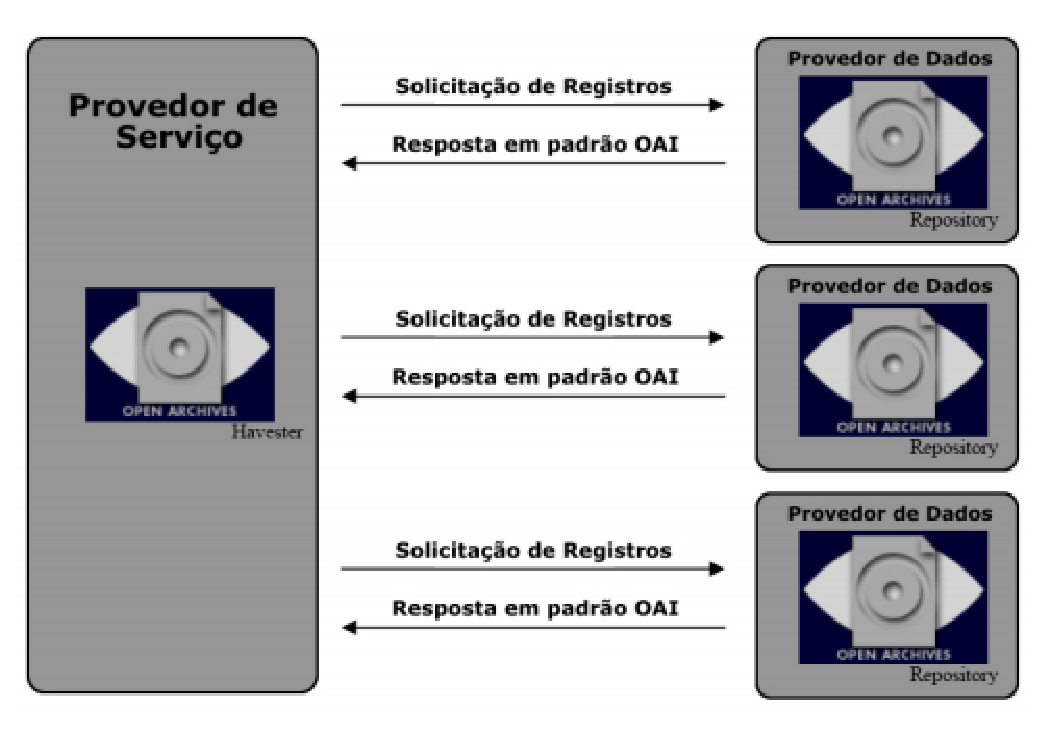
\includegraphics[width=0.9\textwidth]{modelo-oaipmh}
\caption[Modelo de comunicação OAI-PMH entre o portal e os mecanismos]{Modelo de comunicação OAI-PMH entre o portal e os canais de participação. Extraído de \cite{renan2009interoperabilidade}}
\label{fig:modeloaipmh}
\end{figure}

Nessa imagem ilustrada pela figura \ref{fig:modeloaipmh}, os canais de participação conteriam em seus portais, um módulo de biblioteca digital que seria elaborado como produto dessa monografia e distribuído para eles via promoções feitas pelos gestores responsáveis pelo acompanhamento dos canais formais, por exemplo. Com esse módulo acoplado, os canais de participação passam a ter um site pré-configurado e pronto para comportar informações relevantes de uso interno e externo, pelo preenchimento de metadados ou informações tais como telefones de contato, nomes dos conselheiros, reuniões, atas de reuniões e outras informações em formatos variados que possam e necessitem ser catalogadas localmente.

Por outro lado, o portal Participa terá acoplado a si um módulo da biblioteca digital que o tornará um provedor de serviços capaz de interagir com os provedores de dados e coletar metadados essenciais sobre cada um desses provedores de dados, por meio do protocolo de harvesting OAI-PMH. Dessa forma, o Participa poderá auxiliar os canais de participação na organização de seus conteúdos de informação e, ao mesmo tempo, poderá ser um provedor de informações atualizadas sobre os diversos canais de participação, uma vez que as colheitas de dados nos provedores podem ser feitas em qualquer instante desejado. Vale lembrar que o OAI-PMH foi preferido em relação aos outros padrões, como é o caso do Z39.50, porque permite escalabilidade e uma maior liberdade de troca de informações e uma interoperabilidade com baixo grau de envolvimento entre as partes, preservando, dessa forma, a autonomia de cada um dos canais de participação. No caso do OAI-PMH, este padrão foi escolhido já como padrão a ser utilizado para implementação. 

No entanto, para viabilizar essa solução, é importante que, após definida a interface da biblioteca digital, haja uma campanha de distribuição dessas bibliotecas entre os canais de participação interessados, preferencialmente criando-se elementos de motivação que incentivem a adoção máxima desse ambiente de organização de conteúdos e interoperabilidade.

\section{Adaptando o Noosfero para um Provedor de Serviços}

Para viabilizar a construção desse módulo OAI-PMH no Noosfero que utiliza a linguagem Ruby, vista na seção \ref{sec:linguagemruby}, existem alternativas como a gema (\textit{gem}) OAI \footnote{Maiores Informações em: \url{https://github.com/code4lib/ruby-oai}}, que implementam várias funcionalidades entre provedores de dados e serviços pertencentes ao padrão do OAI. No caso do Participa.br, os provedores de dados vão utilizar os protocolos já implementados pelos softwares de bibliotecas digitais e no Noosfero utilizado pelo Participa.br será implementado um plugin, visto na seção \ref{sub:arquiteturaplugin} que irá utilizar a implementação do OAI.

A escolha dessa implementação ser feita em um plugin, deve-se ao fato da necessidade de transformar o Participa.br em uma biblioteca digital seja exclusiva do Participa.br neste primeiro momento. No entanto, nada impede de outras instâncias utilizem esse plugin.

\section{Proposta de interface para a biblioteca digital}
\label{sub:prototipo_biblioteca}

Tomando como referência os levantamentos de software descritos no Anexo \ref{Att:anexobibliotecas} deste documento e nos softwares apresentados na sub-seção seguinte, foi elaborada uma ideia inicial sobre uma biblioteca digital de participação social na intenção de prover, numa estrutura única, os requisitos de sistematização e catalogação colocados na descrição desse produto.
 
Dentre os softwares testados (vide Anexo \ref{Att:anexobibliotecas} deste documento), houve dúvidas entre se utilizar o Greenstone ou o Omeka como infra-estrutura básica para construção da biblioteca digital de participação social e do protótipo que seria apresentado nesse documento. Por esse motivo, foram feitas customizações nesses dois ambientes a fim de identificar elementos que pudessem balizar a escolha, tais como facilidade de uso, características relevantes para o contexto da biblioteca, dentre outros.

As funcionalidades do Greenstone, do Omeka e dos demais softwares testados estão melhor descritas no Anexo~\ref{Att:anexobibliotecas} deste documento. Além disso, outros softwares de bibliotecas digitais foram investigados e estão listados nesse mesmo Anexo.

No protótipo de biblioteca digital foram inseridas todas as informações consideradas relevantes e de acordo com as definições que foram listadas no Capítulo \ref{cap:bibinterop}. No Anexo \ref{Att:catalogomecanismos} foram colocados apenas alguns exemplos de canais de participação para que se possa ter uma ideia do material disponível. A eficiência de localização e busca de dados sobre participação pode ser experimentada com uso deste protótipo de biblioteca digital criado. 

\subsection*{Protótipo das telas}

Para o protótipo apresentado aqui, o Omeka foi escolhido por ser bastante simples em questões de configuração e customização, pois utiliza tecnologias recentes como CSS3 e HTML5 em várias partes de seus temas. No entanto, na versão final desse trabalho pretende-se avaliar outros ambientes para garantir a melhor escolha para o produto de catalogação. 

\subsection*{Informações gerais}

Foi definido um cabeçalho de acordo com e-MAG (\citeyear{emag2013usabilidade}), que é uma série de passos e recomendações para que os portais brasileiros sejam implementados de forma padronizada, de fácil implementação, coerente com as necessidades brasileiras e em conformidade com os padrões internacionais. A primeira versão do e-MAG foi disponibilizada para consulta pública em 18 de janeiro de 2005 e a versão 2.0 já com as alterações propostas, em 14 de dezembro do mesmo ano. Atualmente, o e-MAG encontra-se na versão 3.1 (última versão em dezembro de 2013). 

Ainda de acordo com e-MAG (\citeyear{emag2013usabilidade}) foi formulado um cabeçalho, a imagem ilustrada na figura \ref{fig:cab_prototipo} mostra o mesmo.

%Imagem Cabeçalho
\graphicspath{{figuras/prototipo/}}
\begin{figure}[H]
\centering

\includegraphics[width=1.0\textwidth]{cabecalho}
\caption{Cabeçalho da interface da biblioteca de participação social.}
\label{fig:cab_prototipo}
\end{figure}

No menu existem várias opções de acessibilidade, que ajudam os usuários portadores de necessidades acessar de forma mais facilitada a biblioteca de mecanismos formais de participação.

Para rodapé apresentado na figura \ref{fig:rodape_prototipo} foi utilizado o padrão que há no portal Participa.br, visto que a idéia é fazer que o usuário não perceba que ele está utilizando outro software. Como complemento do rodapé, existe uma referência para o site oficial do Brasil, outra referência para o site Secretaria Geral da Presidência da República, além da referência ao software utilizado (Omeka) e a licença que está sendo utilizada.

%Imagem Rodapé
\graphicspath{{figuras/prototipo/}}
\begin{figure}[H]
\centering

\includegraphics[width=1.0\textwidth]{rodape}
\caption{Rodapé da interface da biblioteca de participação social.}
\label{fig:rodape_prototipo}
\end{figure}

A figura \ref{fig:vertical_prototipo}, possui um menu vertical onde os usuários possam acessar as funções com mais rapidez e facilidade.

%Imagem menu superior
\graphicspath{{figuras/prototipo/}}
\begin{figure}[H]
\centering

\includegraphics[width=1.0\textwidth]{barra-superior}
\caption{Menu vertical da biblioteca de participação social.}
\label{fig:vertical_prototipo}
\end{figure}

Uma das vantagens do Omeka é a personalização desse menu. Através do painel de administração é possível adicionar e remover opções do menu vertical. Existem vários tipos de customização para o menu vertical, entre eles, podemos adicionar links para visualizar todos os itens disponíveis da biblioteca (Ver itens), assim como especificar todos os itens de uma só coleção (Conselhos, Conferências e Ouvidorias). Uma página sobre, que vai conter todas as informações sobre a biblioteca digital e uma busca avançada, onde o usuário vai poder realizar uma busca mais refinada.

\subsection*{Página inicial}

A página inicial contém uma descrição sobre a biblioteca digital. Na figura \ref{fig:inicial_prototipo} é apresentada uma sugestão inicial de como funcionará a biblioteca de mecanismos formais de participação do Participa.br, assim como uma descrição de cada parte da página.

%Figura 3.8 – Descrição de uma coleção na biblioteca do Participa.br.
\graphicspath{{figuras/prototipo/}}
\begin{figure}[H]
\centering
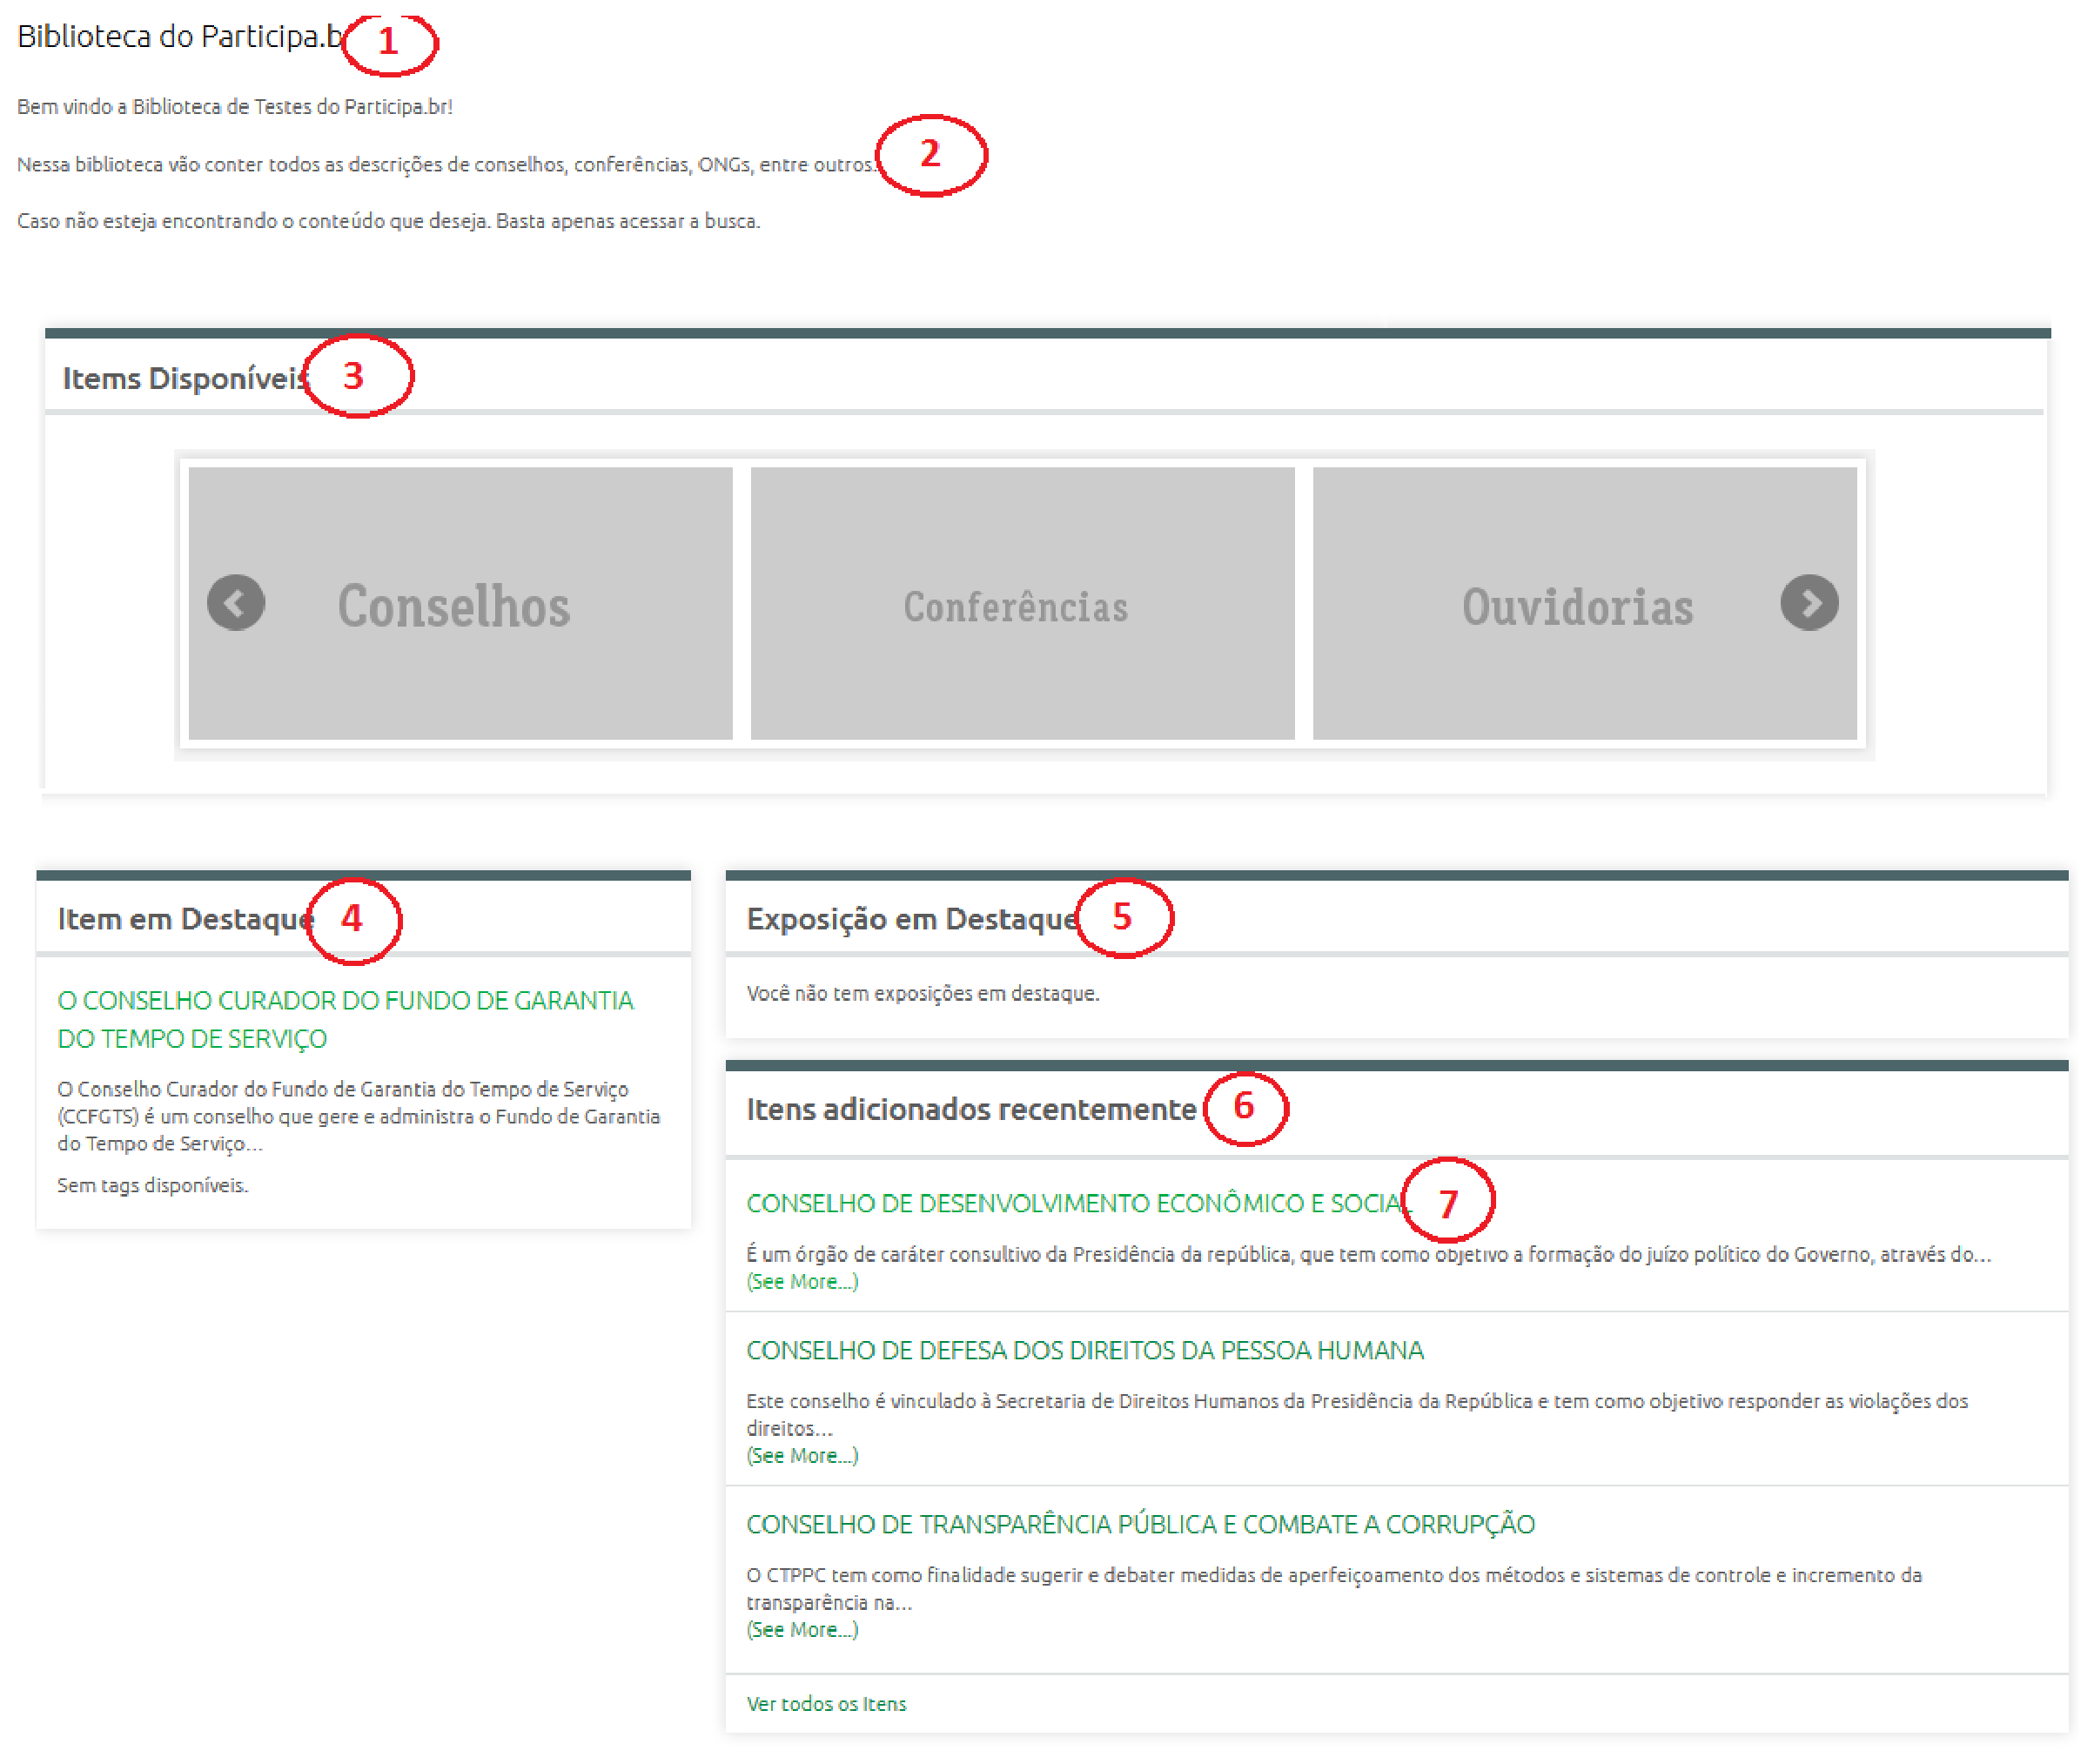
\includegraphics[width=0.9\textwidth]{pagina-inicial}
\caption{Descrição de uma coleção na biblioteca do Participa.br.}
\label{fig:inicial_prototipo}
\end{figure}

\begin{itemize}
	\item \textbf{1 – Título da biblioteca} – Nessa parte é informado o título da biblioteca. Esse título é informado através do painel de administração da ferramenta.
	\item \textbf{2 – Descrição da biblioteca} – Contém uma pequena descrição do objetivo daquela biblioteca para que o usuário possa entender mais sobre a mesma.
	\item \textbf{3 – Menu Slider em jQuery} – Esse menu funciona como acesso rápido para que os usuários possam acessar as coleções de canais formais (Conferência, Conselhos e Ouvidorias). Caso sejam adicionados novos canais formais, o menu alterna entre eles.
	\item \textbf{4 – Itens em Destaques} – Local onde os canais que estão tendo algum tipo de evento naquele determinado dia/semana/mês, pode ser colocado reuniões, encontros, mutirões, entre outros.
	\item \textbf{5 – Exposição em Destaque} – Local onde ficam exposta exposições. Uma exposição é composta por itens que possuem assuntos correlatos, por exemplo, é possível juntar o Conselho Nacional de Saúde, a Conferência Nacional de Saúde e a Ouvidoria do Ministério da Saúde e criar uma exposição chamada saúde.	
	\item \textbf{6 – Itens Adicionados Recentemente} – Nesse etapa, podemos visualizar os itens que acabaram de ser atualizados, isso também ajuda o usuário a perceber a movimentação do portal em relação a atualizações.
	\item \textbf{7 – Listagem de um item na biblioteca} – Nessa listagem os usuários podem verificar o item brevemente. No entanto ao clicar no título é possível acessar o item e todas as suas informações.
\end{itemize}

\subsection*{Acesso a um item}

O acesso a um item é realizado acessando uma coleção. que quando acessado, apresenta todos os itens que compõe aquela coleção são apresentadas na sua forma resumida, conforme será visto na figura \ref{fig:descricao_prototipo}

%Figura 3.9 – Detalhamento de um coleção na biblioteca digital.
\graphicspath{{figuras/prototipo/}}
\begin{figure}[H]
\centering
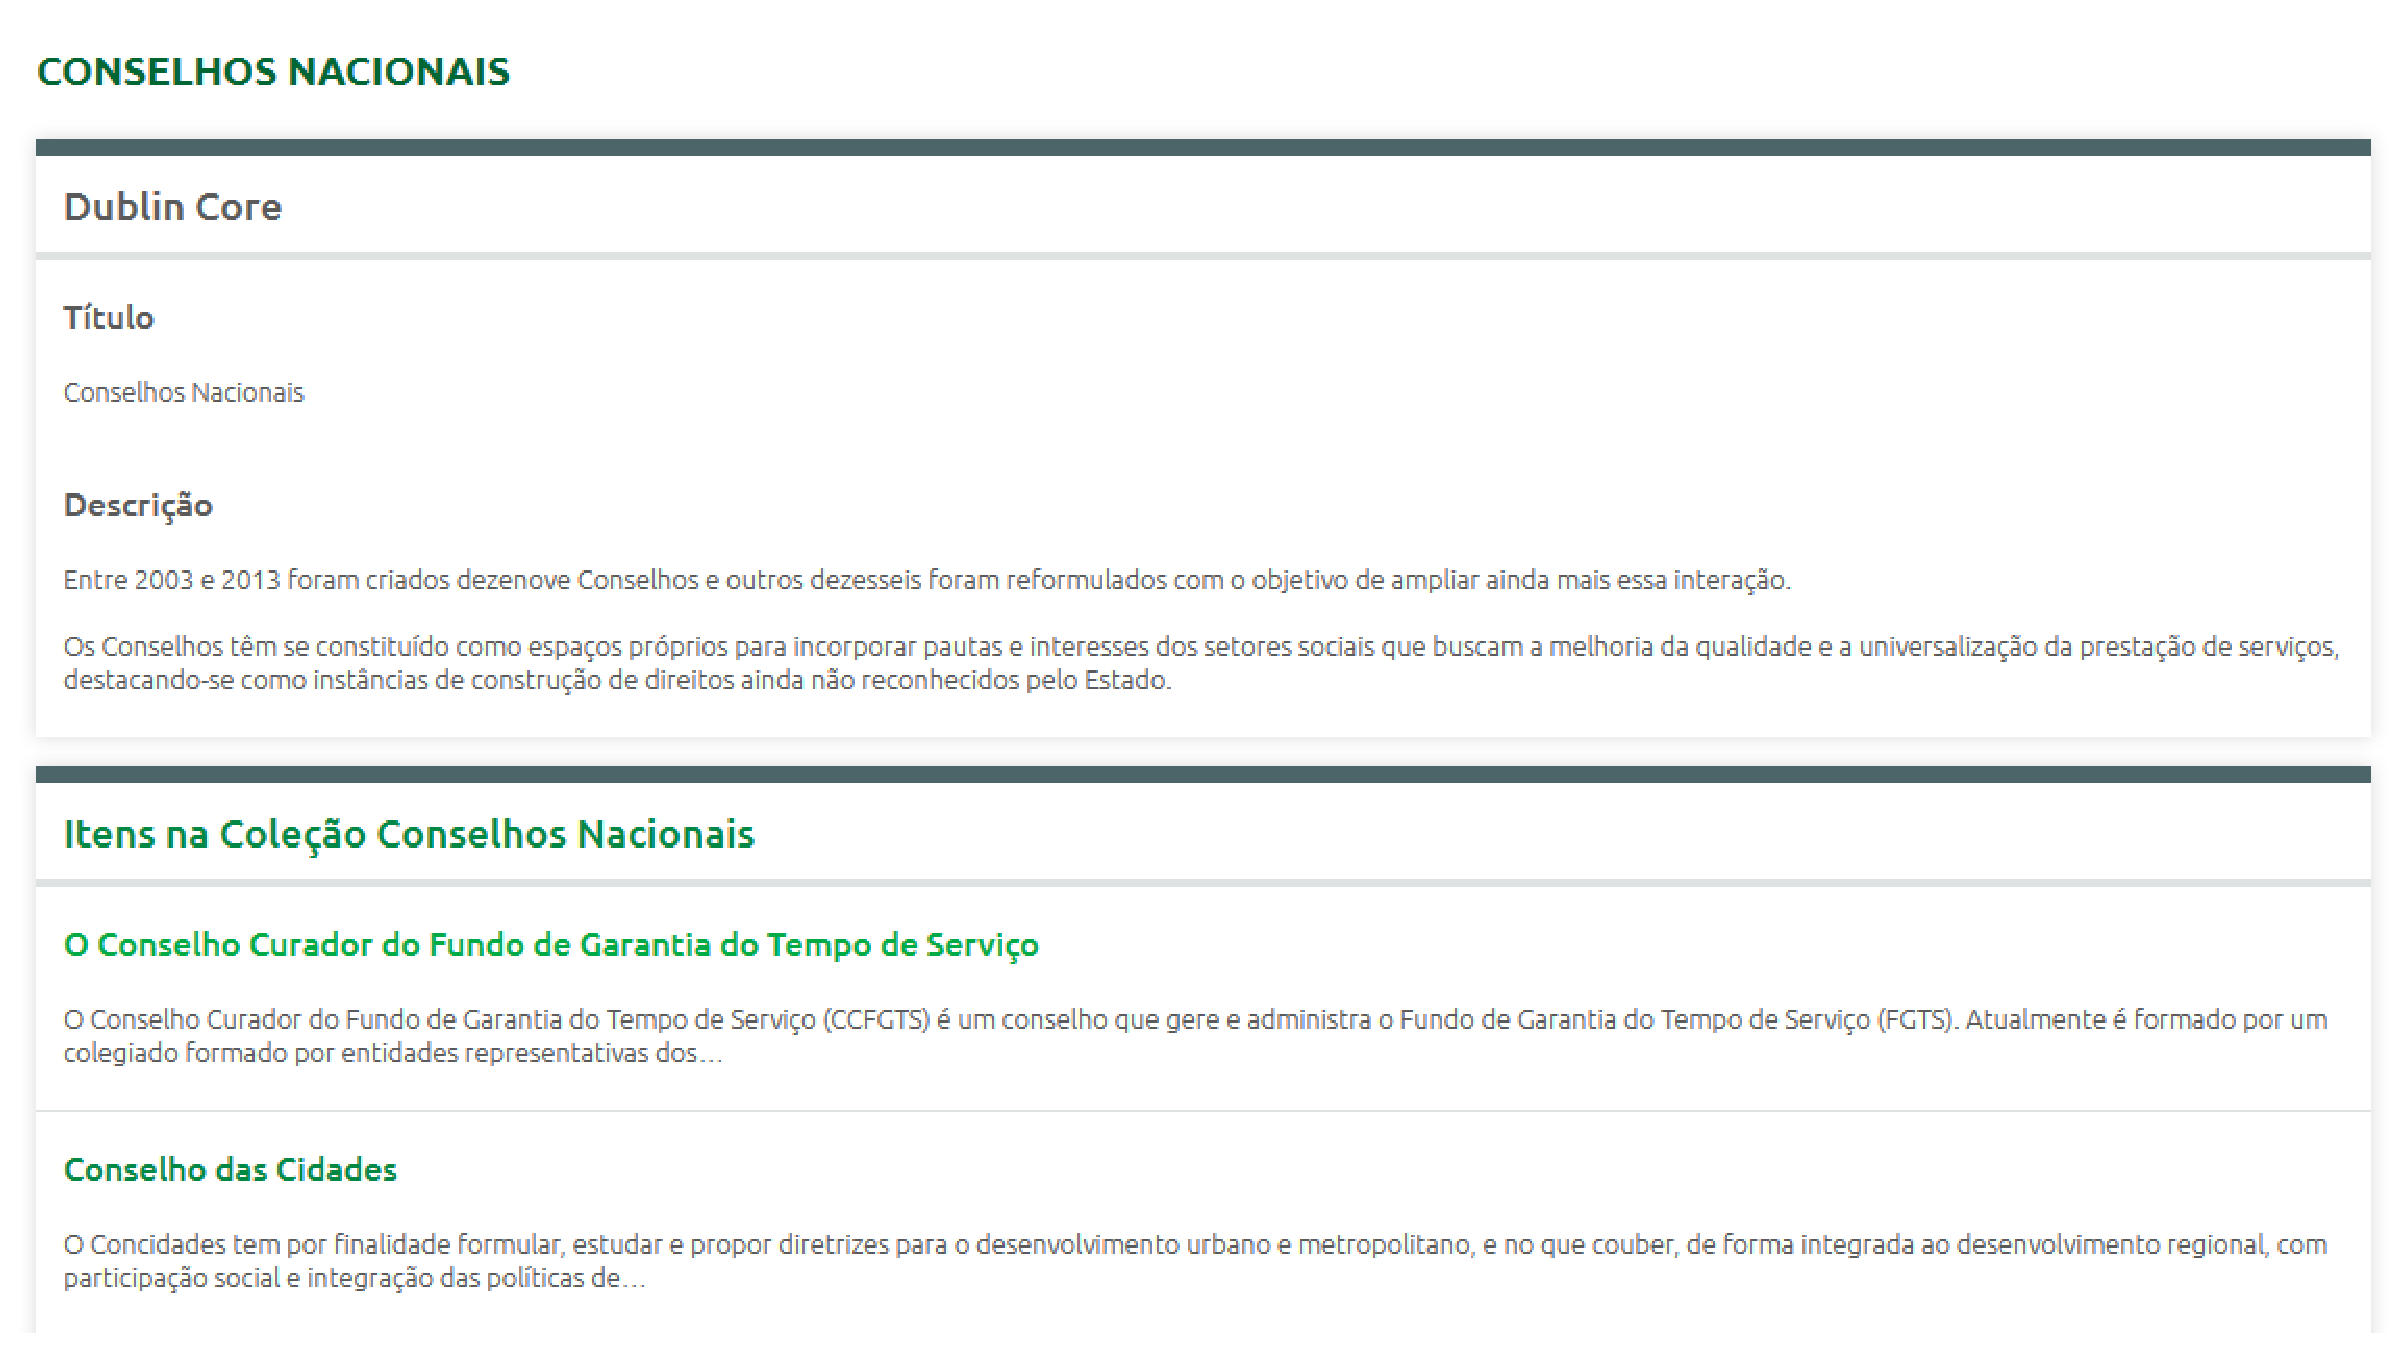
\includegraphics[width=1.0\textwidth]{descricao-colecao}
\caption{Detalhamento de um coleção na biblioteca digital.}
\label{fig:descricao_prototipo}
\end{figure}

Ao acessar um item da coleção acessada, são informados todos os metadados cadastrados para aquele item. No caso da biblioteca de mecanismos formais de participação, serão informados todos os dados cadastrados do respectivo mecanismo, seja ele conselho, conferência, mesa de diálogo, entre outros. 

O padrão da ferramenta é informar primeiramente: (i) os metadados do tipo Dublin Core que foram cadastrados e (ii) metadados customizados da ferramenta. Essas informações podem ser visualizadas na figura da figura \ref{fig:descricao_prototipo}.

O Omeka fornece plugins para enriquecer a visualização. Com isso é possível adicionar geolocalização através do Google Maps, pré-visualização de documentos no estilo Google Docs e Microsoft OneDrive \footnote{Maiores maiores detalhes em \url{Vhttp://pt.wikipedia.org/wiki/Microsoft\_OneDrive.}}, além de extração de PDFs em textos pesquisáveis.

Adicionalmente, pode-se enriquecer a visualização da página através do plugin Exhibit Builder 3.0, que é disponibilizado na parte de plugins do Omeka \footnote{Maiores maiores detalhes em \url{https://omeka.org/add-ons/plugins/}}. Através desse plugin é possível definir um esqueleto para a visualização dos items sem a necessidade de intervir no código fonte, logo é possível definir um esqueleto para a catalogação de um canal formal e replicar nos demais.

%Figura 3.10 – Descrição de um item na biblioteca do Participa.br.
\graphicspath{{figuras/prototipo/}}
\begin{figure}[H]
\centering
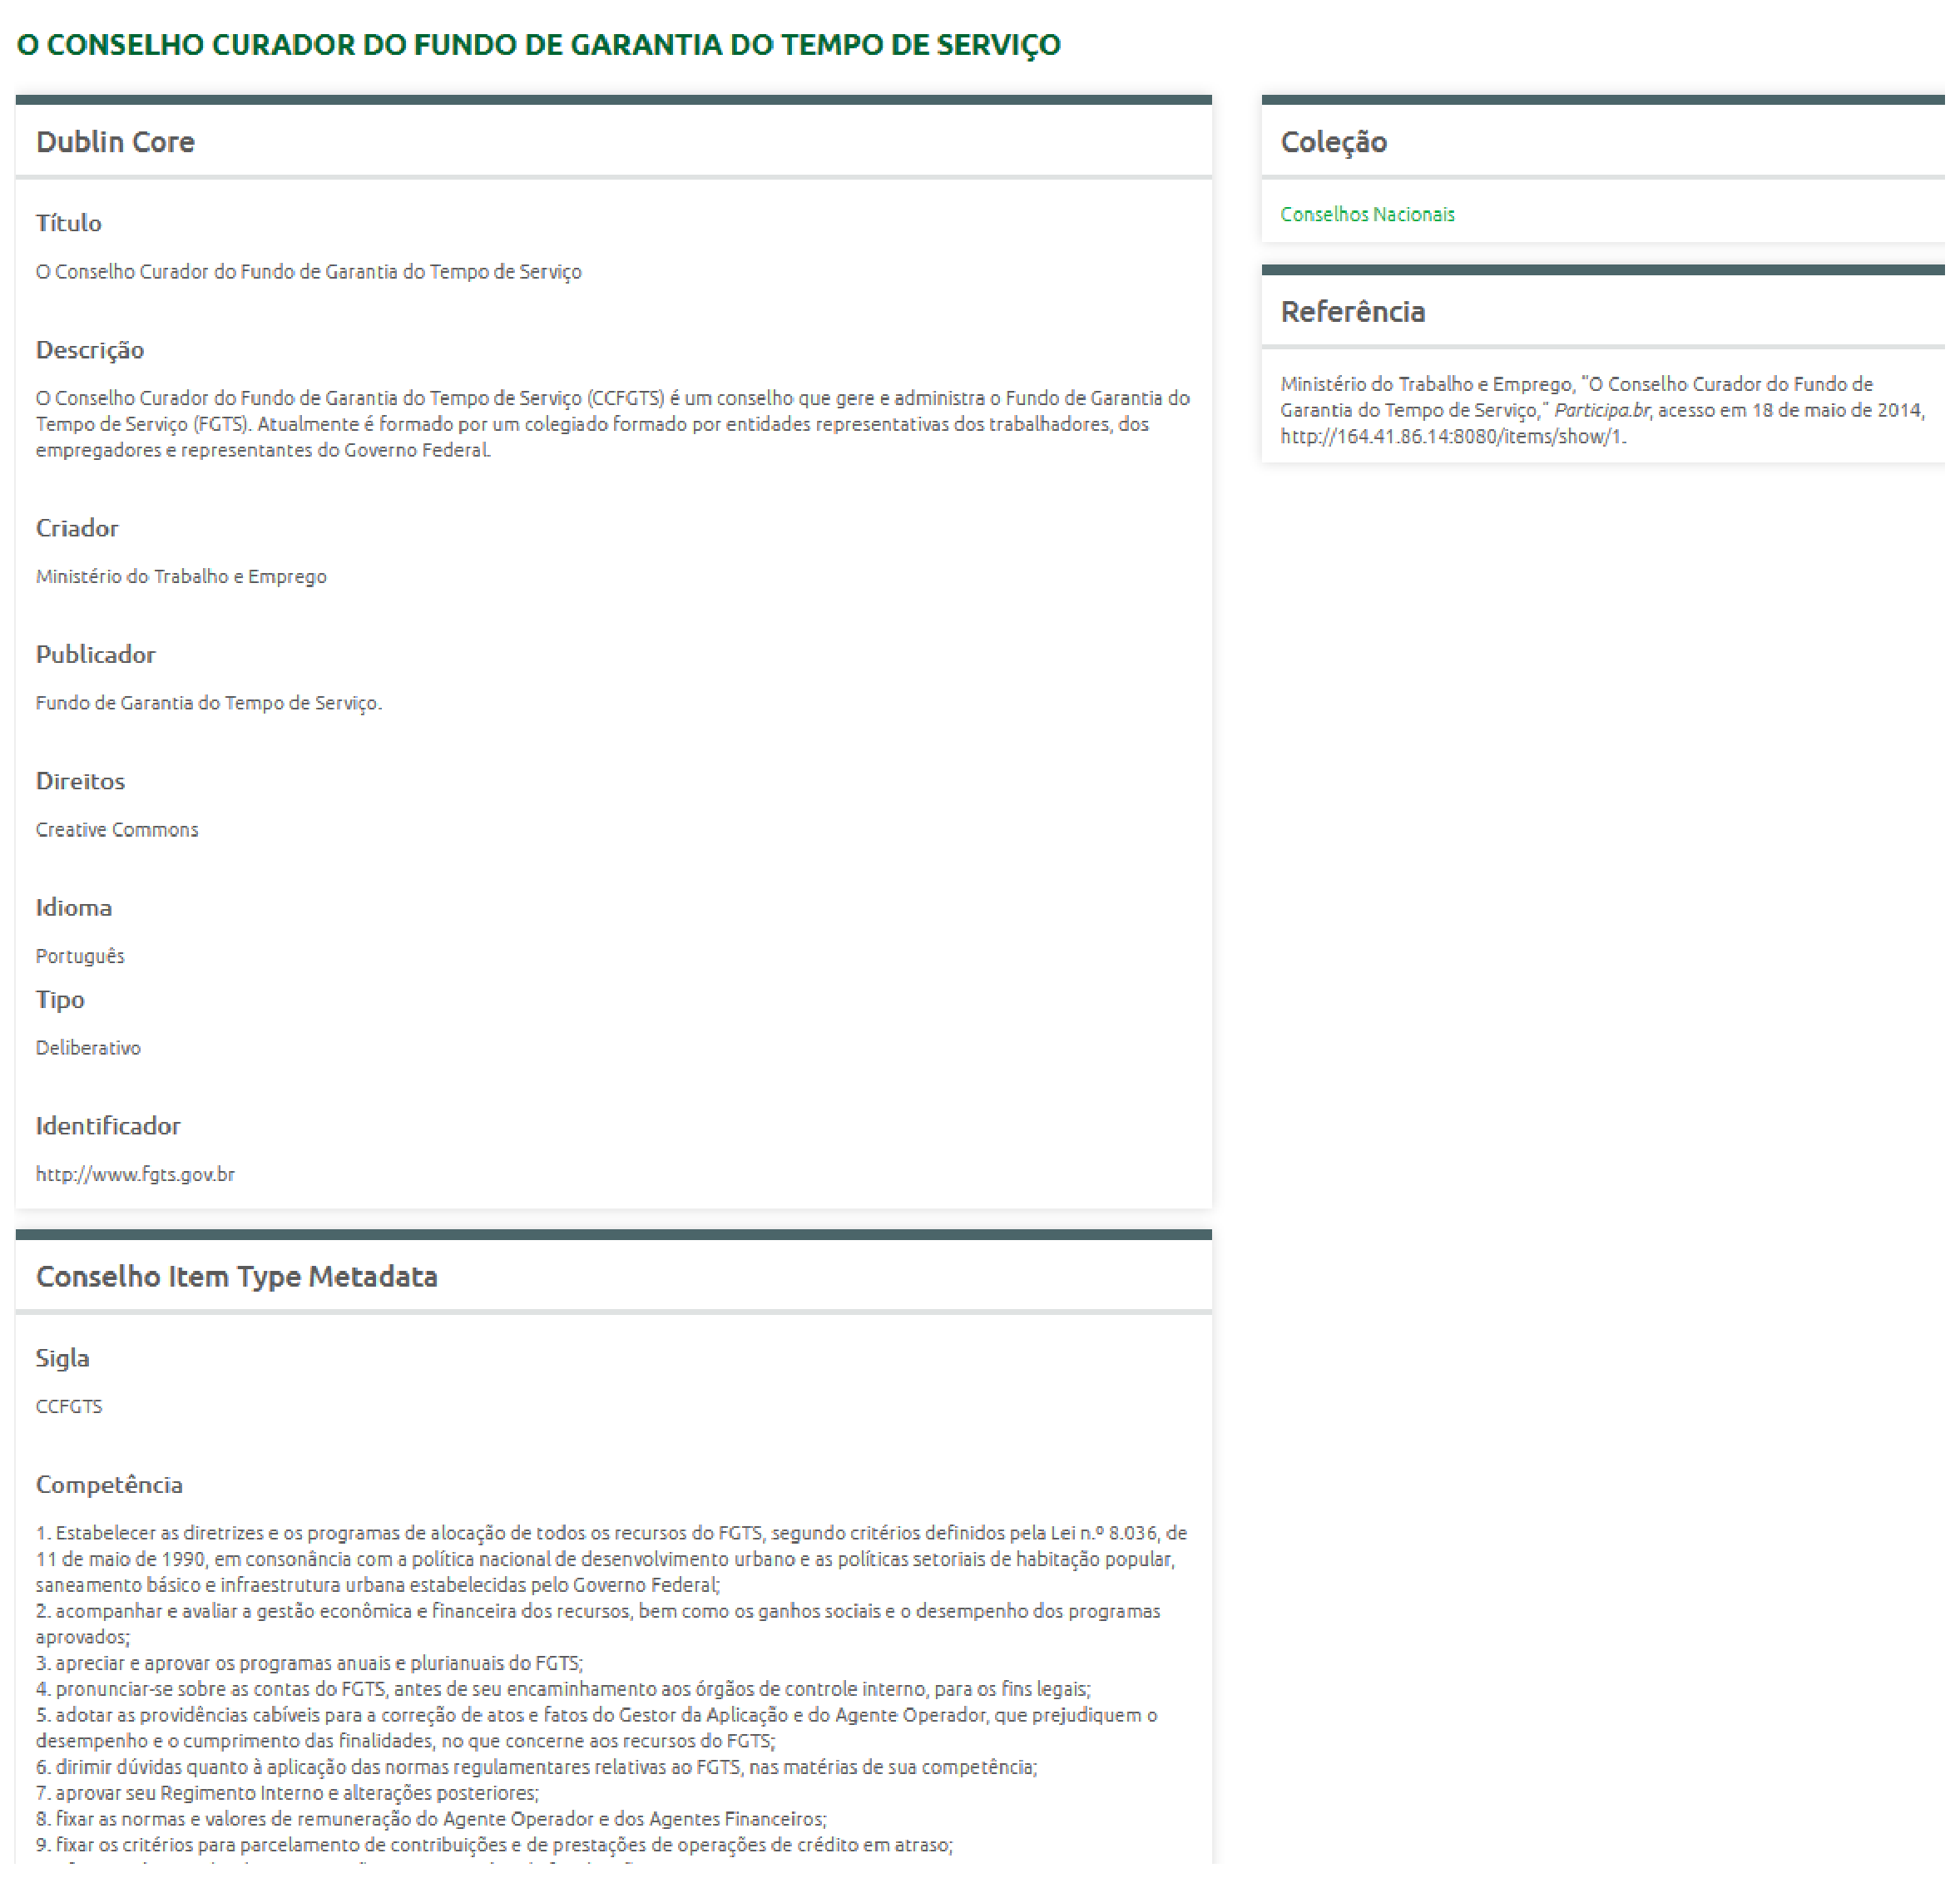
\includegraphics[width=1.0\textwidth]{descricao-item}
\caption{Descrição de um item na biblioteca do Participa.br.}
\label{fig:descricao_prototipo}
\end{figure}

\subsection*{Buscas}

A biblioteca fornece duas opções de busca, entre elas, uma busca simples e outra avançada na qual o usuário pode fazer uma busca mais refinada do que se está pesquisando.
Em relação à busca simples, essa pode ser feita diretamente na barra superior do portal, como ilustrado na figura 3.11.

%Figura 3.11 – Busca simples da Biblioteca Digital
\graphicspath{{figuras/prototipo/}}
\begin{figure}[H]
\centering

\includegraphics[width=1.0\textwidth]{cabecalho}
\caption{Busca simples da Biblioteca Digital.}
\label{fig:buscasimples_prototipo}
\end{figure}

Nesse caso, o usuário pode fazer sua busca diretamente no cabeçalho da biblioteca digital do Participa, que contém as informações sobre redes sociais e opções de acessibilidade, além da "barra Brasil". Quando o usuário digita algo, o sistema realiza essa pesquisa comparando a palavra digitada com todos os textos dos canais formais (incluindo arquivos, caso seja escolhido o plugin), contendo a palavra pesquisada. Essa pesquisa, no entanto, não filtra nenhum tipo de metadado. 

A partir da barra vertical da biblioteca de canais formais do Participa.br é possível acessar a busca avançada, em que os usuários podem realizar busca filtrando os metadados, escolhendo determinada coleção (ouvidoria, conselho, conferência, etc.), entre outros.

Existe uma série de combinações que podem ser feitas para que o usuário consiga encontrar o seu conteúdo de maneira mais fácil. No caso do servidor de testes utilizados para fazer essa biblioteca, a busca está disponível no endereço: /items/search. Nas figuras que se seguem estão representadas as telas com sugestões de funcionamento da busca, assim como a descrição de cada filtro de busca.

%Figura 3.12 – Tela de busca Avançada da Biblioteca Digital
\graphicspath{{figuras/prototipo/}}
\begin{figure}[H]
\centering
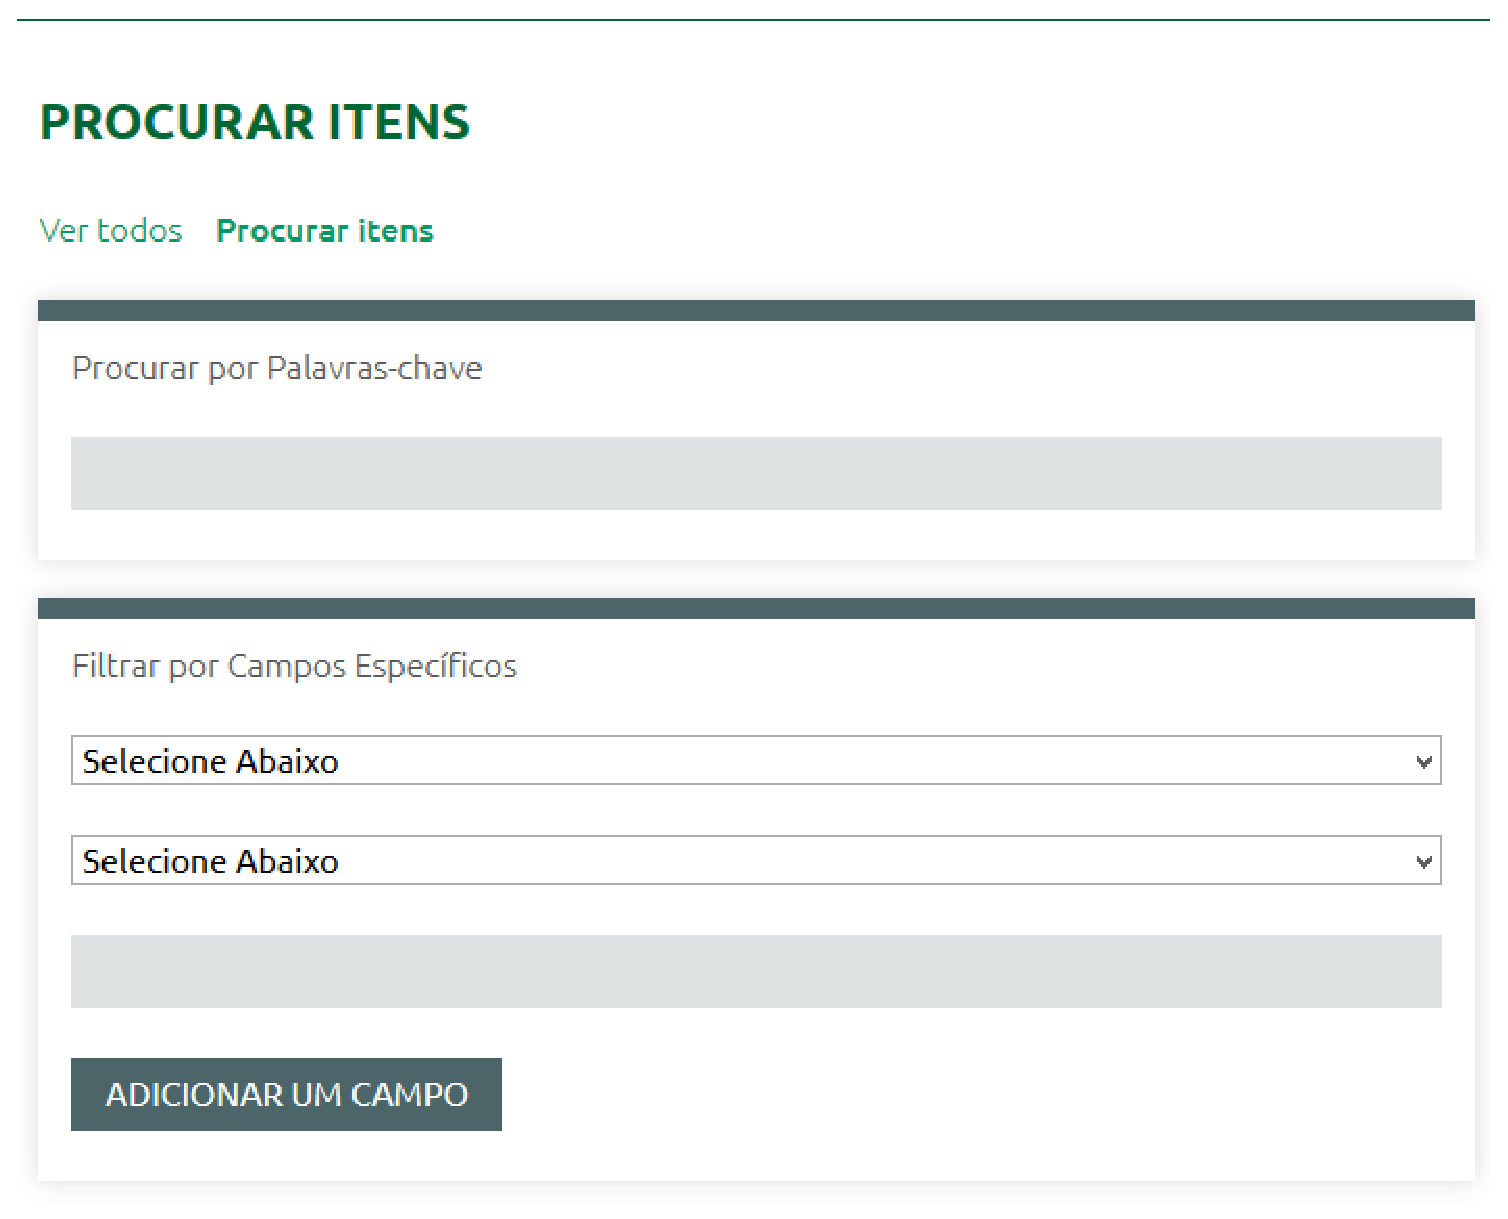
\includegraphics[width=1.0\textwidth]{tela-busca}
\caption{Tela de Busca Avaçanda da Biblioteca Digital.}
\label{fig:buscaavancada_prototipo}
\end{figure}

Essa busca oferece diversos filtros para que o usuário ache somente o que está procurando. Nesses filtros, o usuário pode detalhar a busca por palavras-chaves, coleção, por qual usuário subiu o conteúdo, entre outros. Esses filtros estão detalhados e apresentados nas figuras \ref{fig:buscaavancada_prototipo} a \ref{fig:buscaexposicao_prototipo}.

%Figura 3.13 – Tela de busca por Palavras-Chaves.
\graphicspath{{figuras/prototipo/}}
\begin{figure}[H]
\centering

\includegraphics[width=1.0\textwidth]{busca-palavra-chave}
\caption{Tela de busca por Palavras-Chaves.}
\label{fig:buscachaves_prototipo}
\end{figure}

A busca por palavras-chaves é uma ou mais palavras que resumem os temas principais de um texto. Essas palavras-chaves são um resumo da descrição de cada canal formal na Biblioteca Digital.  Por exemplo, caso o usuário decida pesquisar sobre saúde ou qualquer coisa que remeta ao tema saúde, a biblioteca digital vai apontar para o Conselho Nacional de Saúde e demais relacionados com as palavras pesquisadas. Ela é semelhante a busca simples.

%Figura 3.14 – Tela de busca por Assuntos Específicos.
\graphicspath{{figuras/prototipo/}}
\begin{figure}[H]
\centering
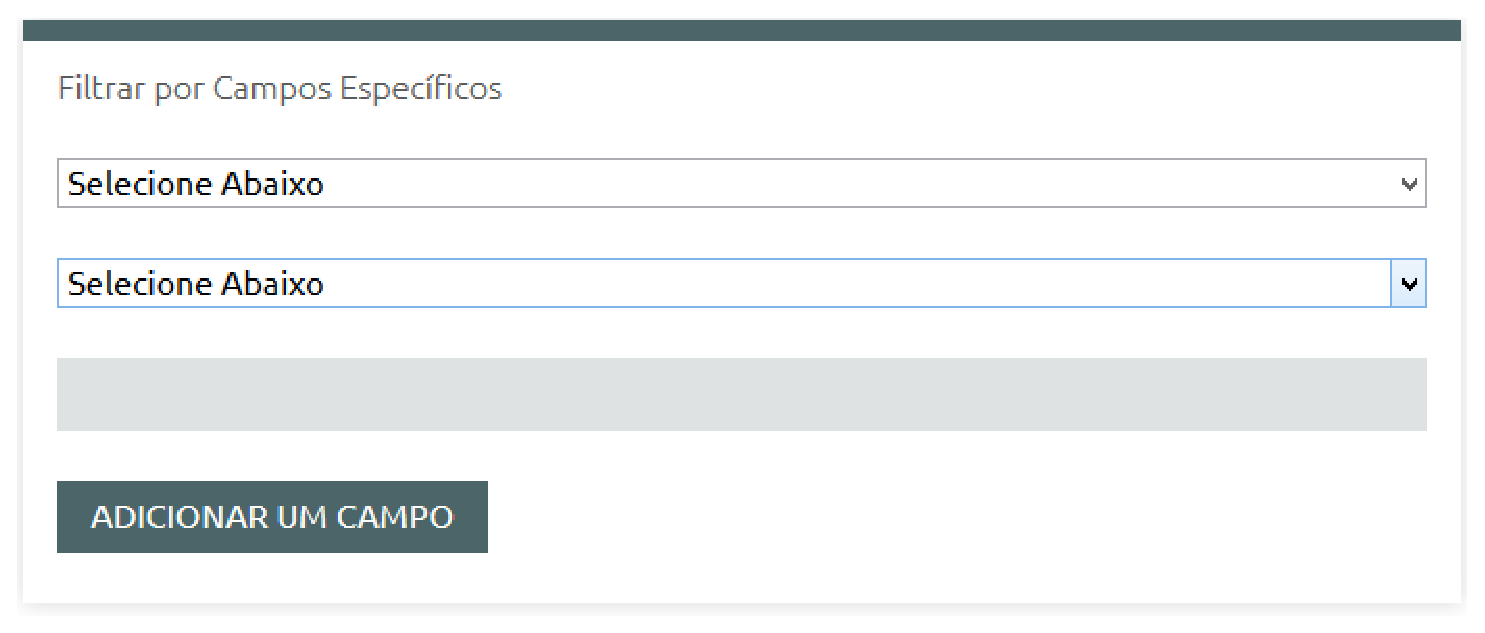
\includegraphics[width=1.0\textwidth]{busca-assunto-especifico}
\caption{Tela de Busca por Palavras-Chaves.}
\label{fig:buscaespecifico_prototipo}
\end{figure}

O filtro de campos específicos é utilizado para o usuário filtrar um metadado específico e verificar: (i) se contém o texto pesquisado, (ii) não contém, (iii) se é vazio, (iv) se não é vazio ou (v) procurar se é exatamente aquela palavra que o usuário está pesquisando. É possível por exemplo, um usuário pesquisar o nome exato de uma pessoa e verificar se ele compõe a gestão de um conselho. Pode-se também verificar se o endereço físico de um mecanismo formal está correto. Também é possível colocar vários filtros, basta para isso adicionar mais campos a sua busca.

%Figura 3.15 – Tela de busca por Identificadores.
\graphicspath{{figuras/prototipo/}}
\begin{figure}[H]
\centering
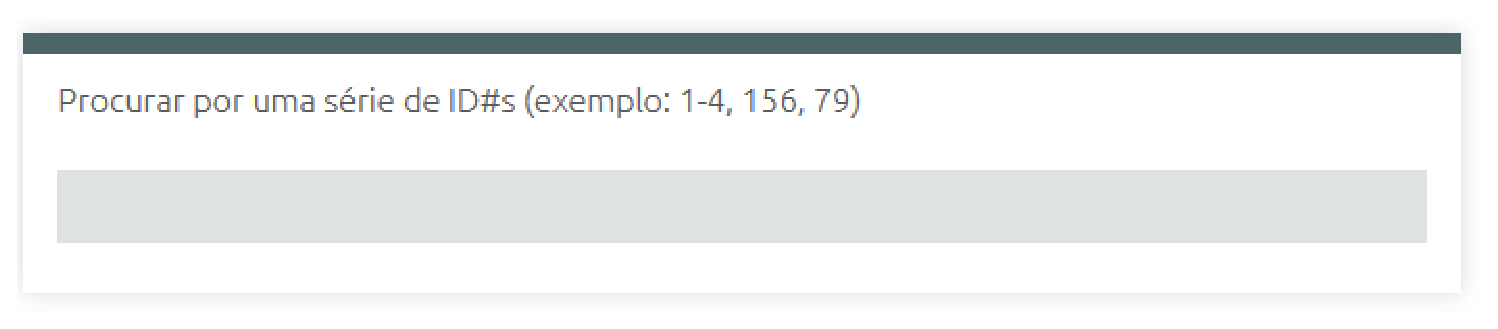
\includegraphics[width=1.0\textwidth]{busca-identificadores}
\caption{Tela de Busca por Identificadores.}
\label{fig:buscaidentificadores_prototipo}
\end{figure}

É também possível fazer busca por identificadores. Nessa caso, cada entrada na biblioteca digital, seja ela um conselho, ouvidoria, conferências, entre outros, é atribuído um ID único. Esse ID é observado quando se acessa um registro na biblioteca. Analisando o endereço da página ao acessar 'items/show/1' e o número no final do endereço que significa o ID daquele registro. Podemos fazer uma pesquisa filtrando apenas os ID`s que nos interessam. Por exemplo, queremos os 30 primeiros itens, ou um intervalo entre 20 e 30.

Uma outra busca possível é por coleção, conforme apresentado na figura \ref{fig:buscacolecao_prototipo}, no qual se escolhe qual tipo de canal formal se quer que seja pesquisado. Por exemplo, pode-se pesquisar por somente Conselhos, Conferência, Ouvidoria, ONG’s, entre outros.

%Figura 3.16 – Tela de busca por coleção.
\graphicspath{{figuras/prototipo/}}
\begin{figure}[H]
\centering

\includegraphics[width=1.0\textwidth]{busca-colecao}
\caption{Tela de Busca por Coleção.}
\label{fig:buscacolecao_prototipo}
\end{figure}

Isso ajuda caso o usuário deseje procurar sobre a Conferência Nacional de Saúde e não sobre o Conselho Nacional de Saúde, apesar dos dois terem temas semelhantes.

% Figura 3.17 – Tela de busca por tipo de metadado.
\graphicspath{{figuras/prototipo/}}
\begin{figure}[H]
\centering

\includegraphics[width=1.0\textwidth]{busca-tipo-metadado}
\caption{Tela de Busca por Tipo de Metadado.}
\label{fig:buscatipometadado_prototipo}
\end{figure}

A busca por tipo funciona como uma busca por metadados definidos pelo administrador da Biblioteca Digital. Nas seções anteriores, foram definidos um conjunto de metadados para o Participa, como metadados de conselho, metadados de conferência e metadados de ouvidoria. Nessa busca por tipo, é possível escolher cada tipo desses citados anteriormente, conforme apresentado na figura \ref{fig:buscatipometadado_prototipo}.

%Figura 3.18 – Tela de busca pelo criador do conteúdo.
\graphicspath{{figuras/prototipo/}}
\begin{figure}[H]
\centering

\includegraphics[width=1.0\textwidth]{busca-criador}
\caption{Tela de Busca por Criador do Conteúdo.}
\label{fig:buscacriador_prototipo}
\end{figure}

No filtro apresentado na figura \ref{fig:buscacriador_prototipo}, é possível selecionar o usuário que criou aquele conteúdo. Por exemplo, pode-se escolher os conteúdos criados pelo Ministério da Saúde, logo teremos o Conselho Nacional de Saúde, Conferência Nacional de Saúde e a Ouvidoria do Ministério da Saúde.

%Figura 3.19 – Tela de busca por tags.
\graphicspath{{figuras/prototipo/}}
\begin{figure}[H]
\centering
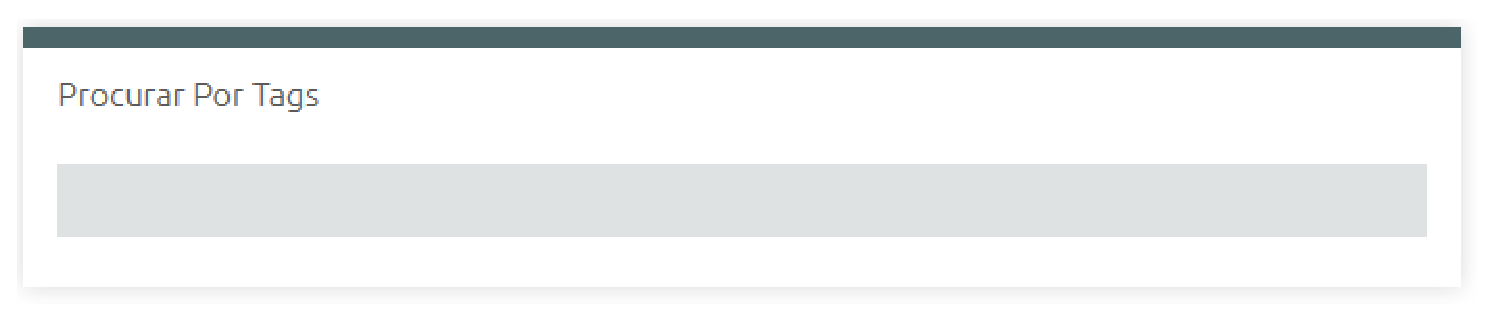
\includegraphics[width=1.0\textwidth]{busca-tags}
\caption{Tela de Busca por Tags.}
\label{fig:buscatags_prototipo}
\end{figure}

Na figura \ref{fig:buscatags_prototipo}, existe uma busca por tag, ou seja, um conjunto de palavras-chaves (relevante) ou termos associados com um registro na biblioteca digital. Nessa busca pode-se escolher uma série de palavras-chaves que são relacionadas ao conteúdo que está send pesquisado. A maioria dessas tags são definidas na descrição de cada canal formal. Nessa busca, pode-se realizar a busca do Conselho Nacional de Educação através das tags relacionadas para esse conteúdo: educação, ensino, escola, aprendizado, entre outros.

%Figura 3.20 – Tela de busca por conteúdo público ou particular.
\graphicspath{{figuras/prototipo/}}
\begin{figure}[H]
\centering
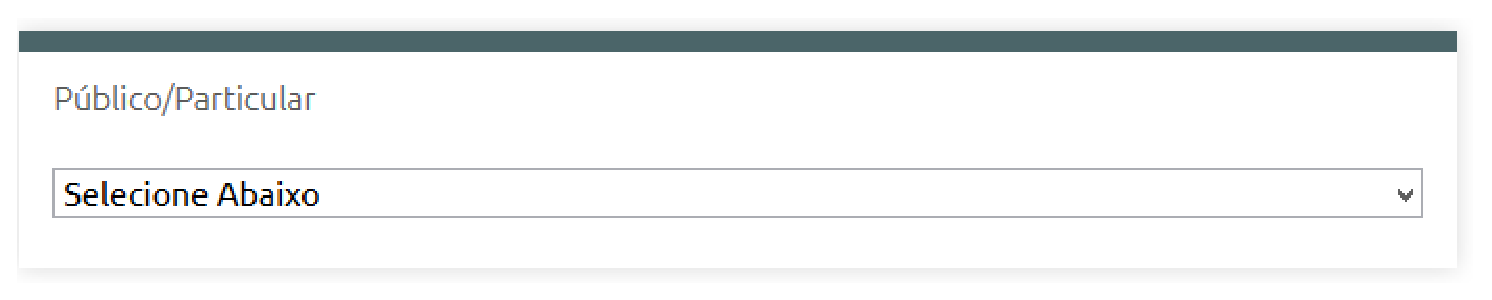
\includegraphics[width=1.0\textwidth]{busca-pub-particular}
\caption{Tela de Busca por Conteúdo Público ou Particular.}
\label{fig:buscaconteudo_prototipo}
\end{figure}

Na figura \ref{fig:buscaconteudo_prototipo}, é apresentada a possibilidade de se escolher conteúdos públicos ou privados. Na biblioteca, alguns conteúdos podem ser públicos (liberado para todos os usuários) ou privados (somente alguns usuários podem acessar). Essa busca é utilizada para escolher entre esses dois tipos de conteúdo, caso o conteúdo particular esteja disponível para o seu usuário.

%Figura 3.21 – Tela por conteúdo destacado ou comum.
\graphicspath{{figuras/prototipo/}}
\begin{figure}[H]
\centering
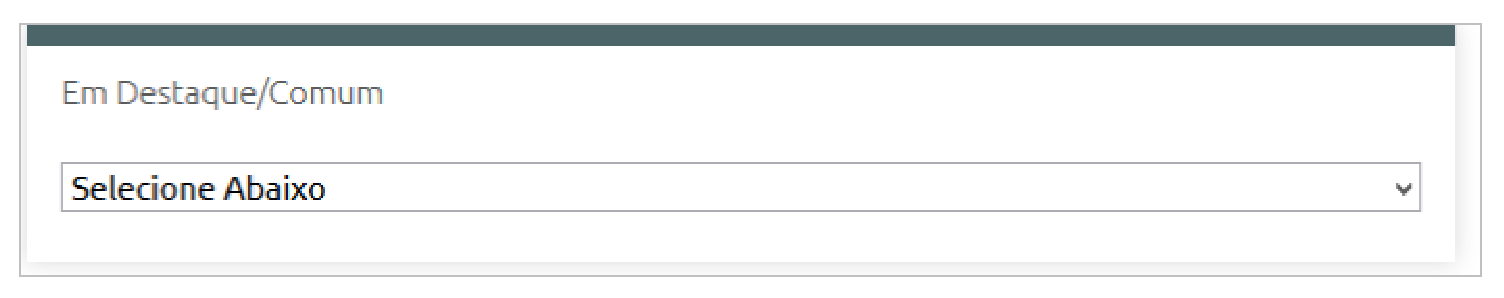
\includegraphics[width=1.0\textwidth]{busca-destacado}
\caption{Tela de Busca por Conteúdo Destacado ou Comum.}
\label{fig:buscadestacado_prototipo}
\end{figure}

Na biblioteca, alguns conteúdos podem ser definidos como destacados ou não (vide figura \ref{fig:buscadestacado_prototipo}), dependendo do nível de acesso do mesmo. Essa busca fornece a busca entre os somente entre os conteúdos destacados ou somente entre os conteúdos comuns.

Busca por exposição.

%Figura 3.22 – Tela de busca por conteúdo sobre exposição.
\graphicspath{{figuras/prototipo/}}
\begin{figure}[H]
\centering

\includegraphics[width=1.0\textwidth]{busca-exposicao}
\caption{Tela de Busca por Conteúdo Sobre Exposição.}
\label{fig:buscaexposicao_prototipo}
\end{figure}

Conforme visto na figura \ref{fig:buscaexposicao_prototipo} pode ser realizadas busca por exposições (itens que tem assuntos correlatos). É possível nessa busca variar entre as mais diversas exposição a fim de refiná-la.

Existe ainda um terceiro tipo de busca que não foi elaborada, mas que permite a utilização do Apache Solr, que é um software livre e plataforma de buscas mais robusta que é um projeto do Apache Lucene. Ele é escrito basicamente em Java e substitui a busca básica em MySQL do Omeka, por uma busca mais refinada. Ela oferece uma busca melhor por textos (com marcações de textos encontrados) um algoritmo melhor de ordenação, melhor busca por metadados dentro dos arquivos de cada descrição de um canal formal, melhor interface para os resultados encontrados.

\subsection*{Resultados da Busca}

Quando é realizada uma busca, a biblioteca digital pesquisa em cada item de seu acervo e verifica se a palavra digitada foi encontrada em algum campo. Essas pesquisas incluem também documentos .pdf, .doc, .html, entre outros, que sejam anexados nas catalogações da biblioteca digital. Na figura \ref{fig:resultante_prototipo}, pode-se notar uma pesquisa utilizando a palavra CCFGTS e seu resultado.

%Figura 3.23 – Tela de resultado da pesquisa.
\graphicspath{{figuras/prototipo/}}
\begin{figure}[H]
\centering

\includegraphics[width=1.1\textwidth]{resultado-pesquisa}
\caption{Tela de Resultado da Pesquisa.}
\label{fig:resultante_prototipo}
\end{figure}

É observado um pequeno resumo da busca no topo da página, contendo o conteúdo pesquisado, ou seja, o termo pesquisado, o tipo de consultado (palavras-chaves, tags, termos exatos, entre outros) e o tipo de registro que deseja encontrar (itens de cada biblioteca, exibições, coleções, entre outros). 
  
Quando é encontrado um item, ele mostra pelo uso de uma tabela, qual foi o tipo de item que foi encontrado e um hiperlink, com o título do item apontado para onde está localizado o item. Quando se clica nesse item, o navegador é apontado para o endereço do canal resultante da pesquisa. Quando se acesso o conteúdo resultante da pesquisa, ele acessa o conteúdo completo daquela pesquisa, conforme imagem ilustrada na figura \ref{fig:resulpesquisa_prototipo}. 

%Figura 3.24 – Tela do item resultante da pesquisa.
\graphicspath{{figuras/prototipo/}}
\begin{figure}[H]
\centering
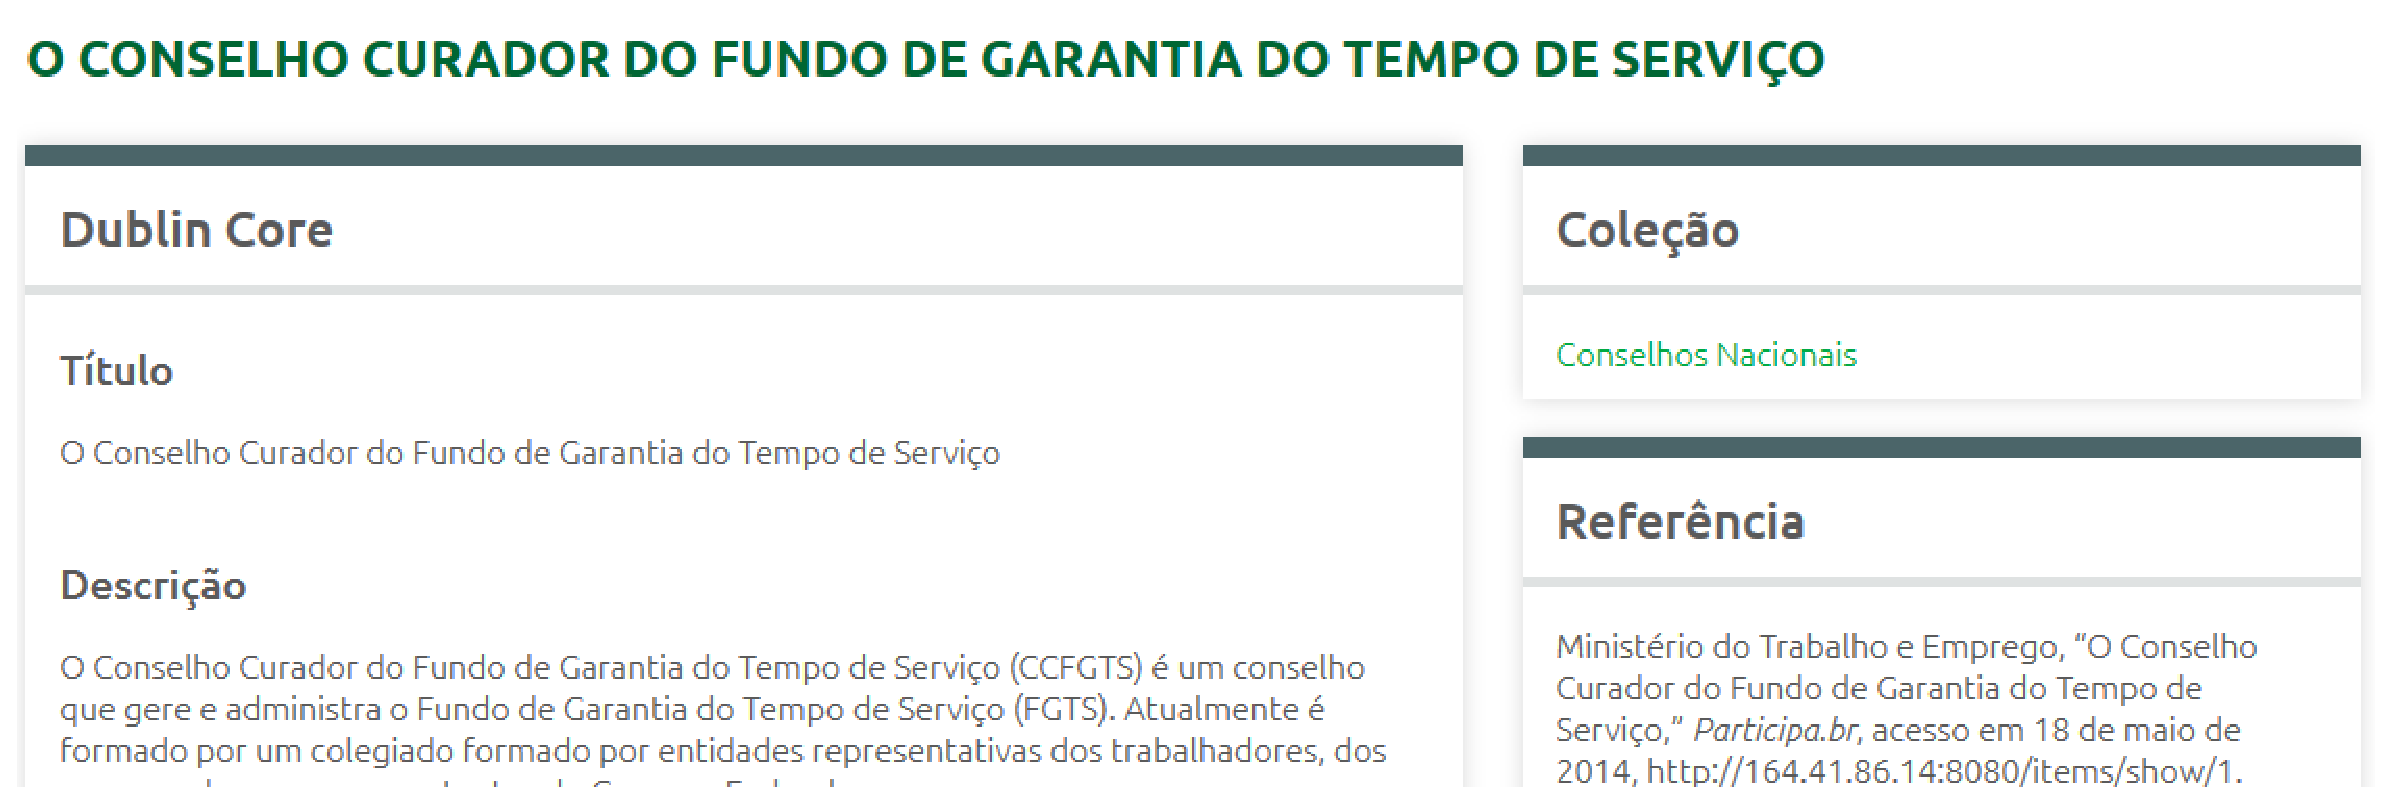
\includegraphics[width=1.0\textwidth]{resultante-pesquisa}
\caption{Tela do Item Resultante da Pesquisa.}
\label{fig:resulpesquisa_prototipo}
\end{figure}



